\documentclass[report]{../../custom}
\begin{document}
\maketitle

\noindent \textbf{摘要:} 本周工作主要围绕SPHINCS\textsuperscript{+}在GPU平台上的加速实现展开。我们深入阅读并比较了Kim et al.~\cite{Kim2024}、Wang et al.~\cite{Wang2025}与Ning et al.~\cite{Ning2024}三篇文献,探讨了各研究在关键组件并行处理、并行策略设计以及内核融合技术等方面的创新点。文献分析揭示了当前实现中在吞吐量和延迟方面存在的瓶颈,为进一步提升系统性能提供了改进思路,如采用GPU并行HASH函数及动态调整并行度等策略。此外,我们还明确了论文写作的风格要求,为投稿的《IEEE Transactions on Circuits and Systems II: Express Briefs》简报文章做准备。

\vskip 0.5cm

\noindent \textbf{下周计划:}
1) 针对当前SPHINCS\textsuperscript{+}实现中采用的CPU串行HASH函数,设计并实现GPU并行HASH函数,并进行初步性能评估;
2) 探索并实现基于各个组件运行时长的动态并行数调整策略,以期进一步提升整体吞吐量;

\section{论文与代码阅读}

\noindent \textbf{阅读:} 为扩展研究视角并探索创新方向,在深入研读了 \cite{Wang2025} 后,我们进一步阅读了另外两篇论文 \cite{Kim2024} 和 \cite{Ning2024}。GPU平台之所以被选取,主要源于其在并行计算性能上具有显著优势。通过比较这三篇论文的创新点(见表 \ref{tab:innovation}),可以看出,各论文均针对SPHINCS\textsuperscript{+}提出了并行优化方法,但其具体的优化策略各有侧重。

\begin{table}[ht]
\centering
\caption{三篇论文创新点比较}
\label{tab:innovation}
\begin{tabular}{l p{0.70\textwidth}}
\toprule
论文 & 创新点 \\
\midrule
Kim et al.~\cite{Kim2024} & 针对SPHINCS\textsuperscript{+}的\textcolor{blue}{关键组件}(FORS、WOTS\textsuperscript{+}、MSS树)提出并行处理方案,在RTX 3090 GPU环境下实现了吞吐量的显著提升,但因多次CUDA内核调用而存在效率瓶颈。 \\
\addlinespace
Wang et al.~\cite{Wang2025} & 提出了CUSPX框架,结合算法级、数据级与混合\textcolor{blue}{并行策略},引入了创新性的并行Merkle树构建算法和多重负载均衡机制,从而实现了较以往更为显著的性能提升。 \\
\addlinespace
Ning et al.~\cite{Ning2024} & 基于自适应并行策略与\textcolor{blue}{内核融合}技术提出GRASP方案,进一步优化了GPU上SPHINCS\textsuperscript{+}的实现效果,显著提升了整体运行效率。 \\
\bottomrule
\end{tabular}
\end{table}

\noindent \textbf{创新点讨论:}
本研究主要关注两个核心性能指标:\textcolor{blue}{吞吐量}和\textcolor{blue}{延迟}。其中,吞吐量衡量在固定核心数条件下GPU处理签名任务的能力,其效果主要受并行效率(PE)的影响;而延迟则反映了签名任务的并行执行程度。为提升吞吐量,相较于采用静态并行数设置,我们计划根据各组件的运行时长\textcolor{blue}{动态调整并行数},从而进一步提高PE。此外,代码阅读过程中发现目前底层的HASH函数采用CPU串行实现,这在一定程度上制约了并行效率。因此,计划将其替换为GPU\textcolor{blue}{并行HASH函数},以期降低延迟并进一步提升系统性能。

\section{论文写作}

\noindent \textbf{写作风格:} 为向《IEEE Transactions on Circuits and Systems II: Express Briefs》简报投稿,i.e., 该期刊于2022年和2025年分别接受了GPU加速AES和PQC实现方面的研究,为此我们使用GPU加速PQC实现,在其投稿范围内。该简报文章的写作风格要求简洁明了,重点突出,且需在\textcolor{blue}{5页以内}。因此,我们将在写作过程中注重\textcolor{blue}{逻辑严谨}、\textcolor{blue}{重点突出},并在\textcolor{blue}{图表设计}上下功夫,以提升文章的可读性。

\noindent \textbf{具体写作:} 本周主要完成文章的介绍部分,就GPU实现SPHINCS\textsuperscript{+}相关工作进行了梳理,并对本文的动机和创新点进行了阐述。具体见图~\ref{fig:composite}。

\begin{figure}[ht]
\centering
\begin{subfigure}[b]{0.32\textwidth}
\centering
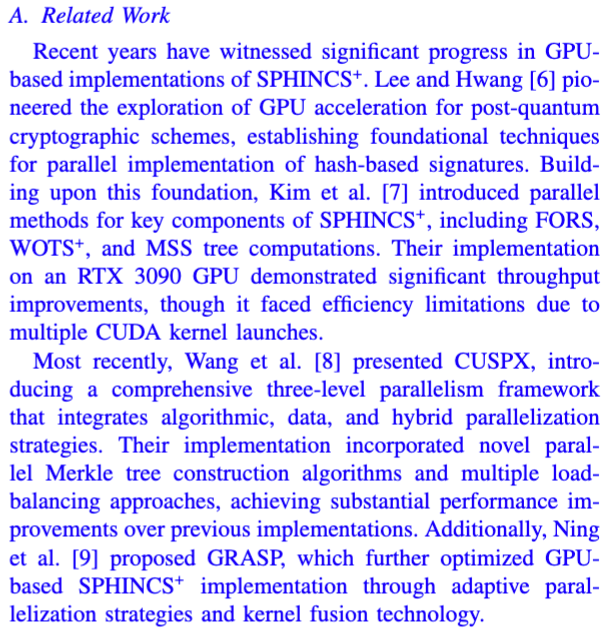
\includegraphics[width=\textwidth]{./fig/relate_work.png}
\caption{相关工作部分}
\label{fig:related_work}
\end{subfigure}\hfill
\begin{subfigure}[b]{0.32\textwidth}
\centering
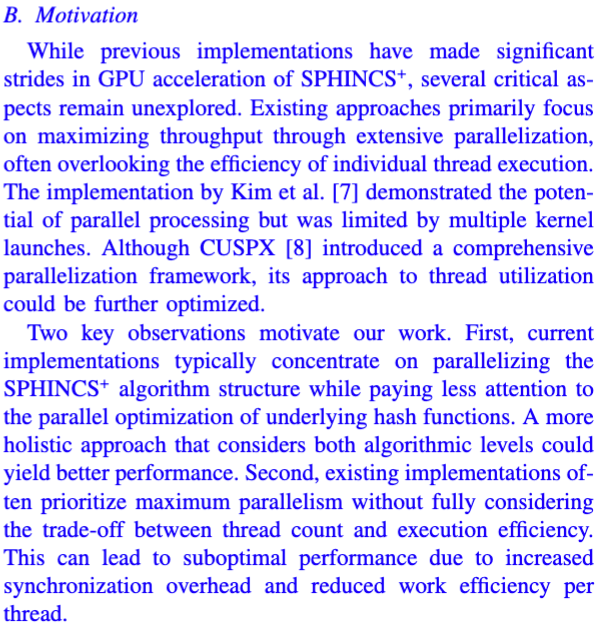
\includegraphics[width=\textwidth]{./fig/motivation.png}
\caption{动机说明}
\label{fig:motivation}
\end{subfigure} \hfill
\begin{subfigure}[b]{0.32\textwidth}
\centering
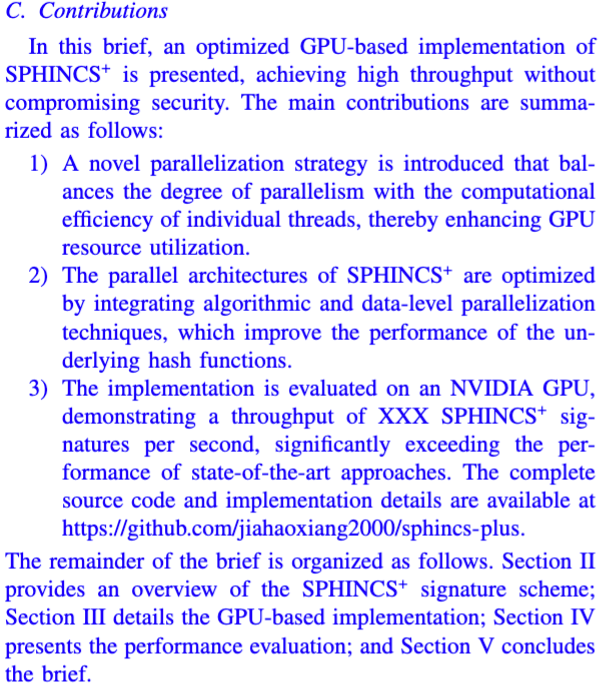
\includegraphics[width=\textwidth]{./fig/contributions.png}
\caption{创新点部分}
\label{fig:contributions}
\end{subfigure}

\caption{组合展示:相关工作、动机与创新点}
\label{fig:composite}
\end{figure}

\bibliographystyle{alpha}
\bibliography{../../paper}

\end{document}